\parindent=0em
\subsection{Lenovo Explorer}
\noindent

La marca Lenovo puso a la venta el dispositivo \textit{Lenovo Explorer} (figura~\ref{fig:lenovoExplorer}) en el año 2017, es un casco de la realidad mixta que se utiliza a través de \textit{Windows Mixed Reality}, es decir, depende de un ordenador para ser utilizado. Este HMD se conecta a través de un cable en Y con conexión HDMI y USB~3.0 y goza de conexión \textit{bluetooth}.\\

Este dispositivo está dotado de sensor de proximidad, giroscopio, acelerómetro y magnetómetro, además, posee dos cámaras para realizar el \textit{tracking} \textit{inside-out}.\\

Por otra parte, tiene un FOV de 110\degree  y una resolución con ambos ojos de 2.880x1.440 píxeles (1.440x1.440 con cada ojo), tiene control de 6 grados de libertad  y su IPD no se puede ajustar viniendo fijo con un valor de 62mm. Este dispositivo no tiene tecnología \textit{hand tracking} ni \textit{eye tracking}, para sustituir el seguimiento de manos se utilizan dos controladores que funcionan con pilas del tipo AA. Su peso es de 380 gramos. 

%https://www.amazon.com/-/es/Lenovo-G0A20001WW-Explorer-Mixed-Reality-Auriculares/dp/B0764GKZ15


\begin{figure}[H]
    \centering
    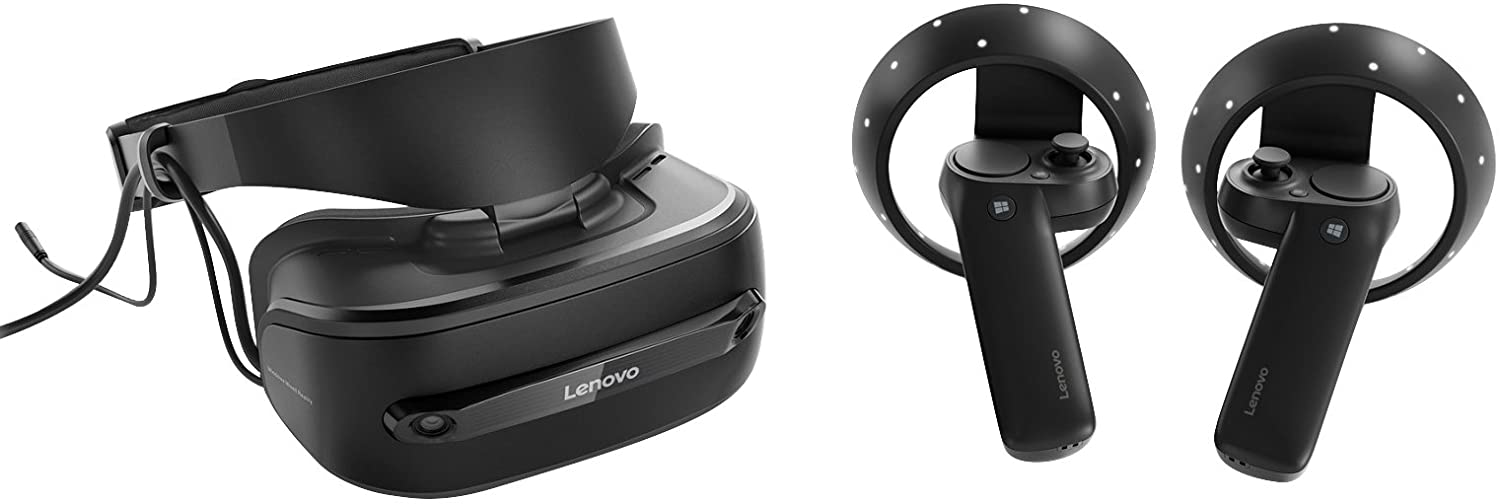
\includegraphics[scale=0.2]{Images/Estado del arte/lenovoexplorer.jpg}
    \caption[Lenovo Explore]{\textit{Lenovo Explore}r\footnotemark.}
    \label{fig:lenovoExplorer}
\end{figure}

\footnotetext{Fuente: \href{https://www.lenovo.com/es/es/smart-devices/virtual-reality/lenovo-explorer/Lenovo-Explorer/p/G10NREAG0A2}{\nolinkurl{https://www.lenovo.com/Lenovo-Explorer/p/G10NREAG0A2}}}
